\chapter{Discussion}
\label{chapter_discussion}
This chapter contains a discussion on how the perspectives are best used and how they can fulfill or replace each other. Further the examined news applications will be classified into different categories and the implementation of the use case will be discussed.

\section{Perspectives}
There are a handful of different perspectives presented in section \ref{perspectives_presentation}, and they all seem to have different purposes and functions in a mobile news application. However there are several of the perspectives presented that in one way or another can overlap each other, or even replace another perspective completely. Some may be combined, and others may be split down into several perspectives. Some screens that are used throughout the different apps, like for instance a category selection screen or search screen, are not classified as a news perspective since it does not contain any information directly from a news article.

At a basis, a mobile news application should at least consist of two perspectives. An entry perspective and a perspective providing more information to an article linked from the entry perspective. The entry perspective should have as a main function to show articles or topics in a clear and lucid manner to be able to present the user with an easy way of understanding what the article or topic is mainly about. If the user finds it interesting and wants to access more information about the article or a given topic, the entry perspective should point to a perspective containing this. Further other perspectives can be added in addition to the two main perspectives to provide a higher navigation hierarchy, or replacing some of them by breaking down into smaller or other types of perspectives serving the same purpose.

A basic news model containing only the two main perspectives mentioned above, could be a simple RSS reader which consists of an RSS perspective as the entry perspective and a web perspective as the perspective holding more information about a single news article. This is an approach that is widely used, but if the developers wanted to extend this model in some way to convey the information in another way, this could be done using some of the other perspectives. For instance, the RSS perspective could be replaced by the event perspective to quickly tell what the article was about, further the event perspective could be linked to a summary perspective to give a little bit more depth to the article before the summary perspective sends the user further down the navigation hierarchy to a full article perspective containing all there is to know about this article.

Some of the perspectives presented could also be combined. The event perspective and the entity perspective could be melted down to one perspective by, for instance, having a view showing the events that the news article concerns, and at the same time highlighting the different entities that are identified in the events that are listed. Further the click of an entity could send the user to a new RSS perspective showing a list of articles that are connected to this entity.

As well as combining perspectives, some perspectives can be broken down into smaller pieces as well. Take, for instance, the full article perspective. This is a perspective that holds a lot of information, and say that the user only wants to access the article's full text, this could be presented as an own perspective, only showing the article's full body text, and excluding all the other information about the article that are not interesting at the given moment, and at some point could be perceived as noise.

It is also important to use the different perspectives where they are best intended and serves the best possible purpose. Presenting a full article perspective as an entry point with an article the user may not be interested in at all, may be perceived as too much information and even noise by the user. Showing a map perspective with no contextual information may be very confusing to the user, not knowing why that pin is placed at that place or what the article is about in the first place.

\section{Mobile News Applications}
Table \ref{table_comparing_apps}, which presents the different news applications that are examined, shows that there are a lot of similarities between the applications. However, each application has some features or is lacking some features, that make them classifiable.

The different applications can be broken down to three main categories, depending on their features and what their main area of focus are. The three categories are recommendation apps, summarization apps and advanced RSS apps, where these names are created solely to try to give an understanding of what the main focus areas or features of the application are.

\subsection{Recommendation Apps}
These are the applications that focuses mainly on giving users the news they think they want, by using some sort of advanced recommendation and personalization technologies, based on the user's explicit and/or implicit feedback. Following are the apps put in this category.

\begin{itemize}
	\item Zite
	\item News360
	\item Prismatic
	\item Use case
\end{itemize}


All these application are put in this category because they all track the user's activity to gain implicit feedback from the user, and some of them also uses explicit feedback for even better user profiling. They all use some kind of advanced recommendation technology to recommend news based on the user profile, and their main focus is on the recommendation technology and providing the user with news that best fits the user profile.

\subsection{Summarization Apps}
These are the applications that focuses mostly on creating quality content for their users, by summarizing and extracting the most important parts of the news articles, and not focusing as much, or at all, on recommending news. Following are the apps put in this category:

\begin{itemize}
	\item Summly
	\item Circa
\end{itemize}

Both Summly's and Circa's main focus are on extracting the most important information from a news article and presenting it to the user. Neither of them have any user profiling or recommendation of news to the user. Both deliver the most trending news and trusts the user to find the news that they want themselves. Summly has the ability to search for and add news categories or topics, while Circa only has a finite set of categories and news articles to choose from. However, with Circa the user can choose to follow different stories, and get notified when a story changes or new information to a story is added.

Even though their put in the same category and their main focus is the same, their approach to create summaries are totally different. Summly uses NLP and machine learning to analyze text and extracting the main content, while Circa has real human editors that creates their summaries.



\subsection{Advanced RSS Apps}
These are the applications that works similarly to normal RSS readers, and does not strive to create content summaries or recommend news on an advanced level, but may include more functionality than a basic RSS reader like proposals to news categories for the users, searching for content, or crawling social sites for content that is shared. Following are the apps put in this category.

\begin{itemize}
	\item Flipboard
	\item Pulse
	\item Wavii
	\item Taptu
	\item Feedly
\end{itemize}

The applications put in this category are applications that neither recommend news based on user profiles or creates summaries for the user. These application can be thought of as advanced RSS readers, which helps the user with getting content, but having the user adding content explicitly. All applications has a certain set of preloaded categories or content the user can choose to add to the news feed, but news are not recommended based on what the user is doing. Some of these applications also has a more social aspect allowing the user to add their social feeds into the application. The news that are delivered to the user are more based on what is hot and trending with regard to most shared on Twitter or Facebook, for instance, than tailoring it specifically for the single user. 

Wavii is somewhat different than the others though, since this application creates events from news content, and present these in a Facebook type of manner, but it still presents news events that are trending and not tailored for the single user.

\section{Use Case Implementation}
The use case application presented in section \ref{use_case_application} were meant to include all of the perspectives described in section \ref{perspectives_presentation} to see how it could be solved in navigational and presentational manner, but this was not feasible at this point due to several factors. How to implement it has been thought of and will be presented in chapter \ref{further_work}.

To sum up how the application's perspectives are implemented in a brief manner, the RSS perspective is presented after the user has chosen recommended news or another category. From the RSS perspective, the user can either go back or open the full article perspective which links to related articles and the map perspective.

The application uses mostly gestures for navigational purposes to save space on the already limited screen size that comes with mobile devices, and buttons are kept to a minimum. This may lead to less intuitive user interface, as mentioned by some of the users when testing the application\footnote{The application was tested on five persons, all male, in the age 21-30, where the test persons used the application for ten to fifteen minutes and afterwards spoke freely of what they thought of the application and how it was to use. Also the application included checkpoints to build statistics of how the application was used.}. 

Some of the users stated that the navigation between perspectives sometimes was counter intuitive, meaning that they were presented with the previous perspective when they wanted to go forward and vice versa. For instance was the category selection screen shown when they wanted to view the full article perspective. This was in most cases quickly adapted, after the application had been used a bit. This can also be reflected by the statistics gathered from the usage of the application (see figure \ref{usecase_usage_stats}), where it shows that the number of times the top stories was shown throughout a month was almost equal to the times the settings screen was shown, which probably was not the user's intention. The navigation scheme in the application may be a bit different as most mobile users probably are used to get new perspectives stacked from the right, as is the scheme in most mobile applications, and not stacked down from the top.

\begin{figure}[!htbp]
\centering
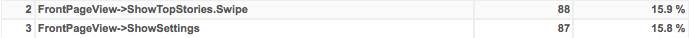
\includegraphics[width=130mm]{GFX/usecase/usageStats.png}
\caption{Statistics from the use case application showing how many times the top stories and settings screen are shown in a month.}
\label{usecase_usage_stats}
\end{figure}

The navigation scheme can be seen as rotated 90 degrees to the left to what is mostly used in the other news applications. Instead of swiping up to scroll down to see more, the user has to swipe left to scroll right to see more news, and instead of bringing new perspectives in from the right, the application stacks them from the top. As this maybe be confusing to some, it is consistently done throughout the whole application and was quickly adapted by most of the users that tested it. To help users to start using the application it also has small pop-ups, explaining how to navigate around the application, the first time it is launched.

It could have been wiser to just follow a well established navigation scheme, as this probably are more intuitive to the user and the testing showed that most of the users testing the application did not pay much attention to the pop-ups, but just started to use the application without reading what the pop-ups said.

The reason that this approach was chosen, was that it was a little different than the other most used design approaches, as well as it suited the swipe-based navigation scheme that was one of the main focuses to follow when developing the application. There are probably a lot of different approaches than could have been followed to design and implement the use case application, like the vertical news feed used in Zite for instance, or the two dimensional scroll views, used in Pulse and Taptu. The main reason the vertical scroll solution, found in Zite, was not chosen, was that it was too main stream, hence to familiar to the common user. A point was to not have a too familiar UI, to see how the navigation scheme developed were to be received at the user's end, without any pre-knowledge of how it would work. The main reason the two dimensional UI approach, found in Pulse was not chosen, was that it appeared too cluttered with too much information displaying on a small mobile screen.

The navigation scheme put aside, the application worked well with the connection between the perspectives and the users stated that the perspectives showed what they was expecting to see in the different perspectives. Again, there was no big surprises to how the information was presented, as all the perspectives used layouts that are pretty common in other applications.











